%!TEX root = ../report.tex

\section{Architectural Patterns}

\subsection{Layer Pattern}
Structure:\\
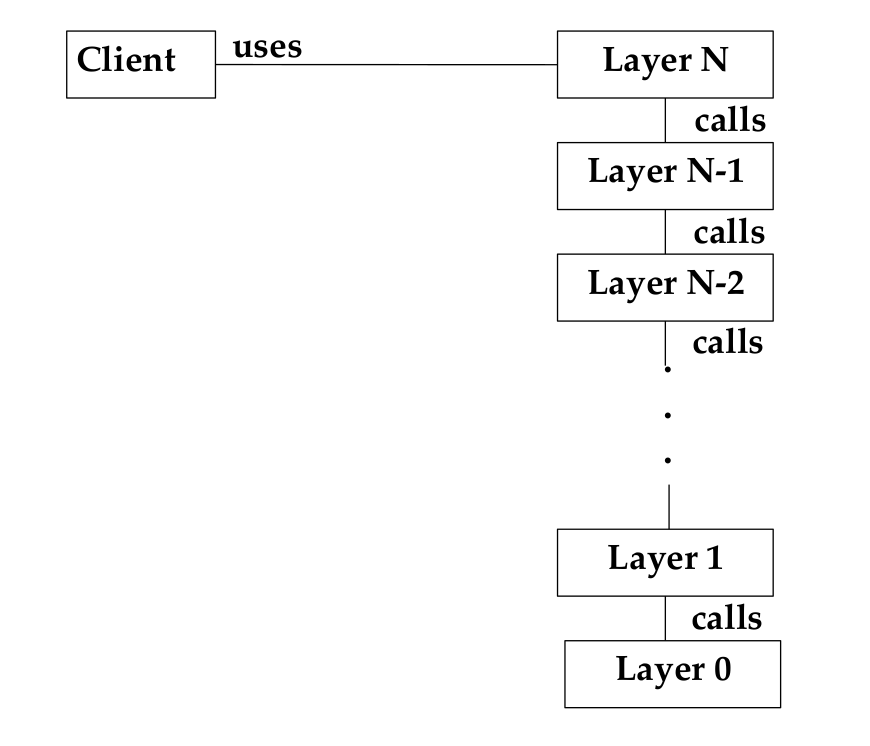
\includegraphics[width=.75\linewidth]{images/pattern_layer.png}
\begin{description}
  \item[Closed Architecture (Opaque Layering):]\hfill \\
    Each layer can only call operations from the layer below.\\
  \item[Open Architecture (Transparent Layering):]\hfill \\
    Each layer can call operations from \textbf{any} layer below
\end{description}

\textbf{5 Steps to Create a Layered Architecture}
\begin{enumerate}
  \item Identify subsystems
  \item Structure the individual layers
  \item Specify the communication protocol between adjacent layers (push/pull)
  \item Decouple adjacent layers
  \item Design an error-handling strategy (try handling errors on lowest possible layer)
\end{enumerate}
\newpage

\subsection{Repository Pattern}
The repository pattern is used to support a collection of independent programs that work cooperatively on a common data structure called the repository.
The control flow is not specified by the pattern.\\
Structure:\\
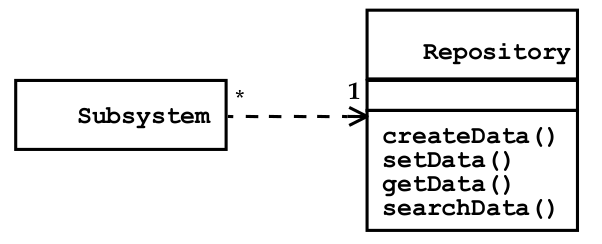
\includegraphics[width=.75\linewidth]{images/pattern_repository.png}
\newpage

\subsection{Blackboard Pattern}
Experts throwing knowledge onto a blackboard (repository) which might be correct or not. Some can be extracted to higher order knowledge and other might be rejected.\\
Structure:\\
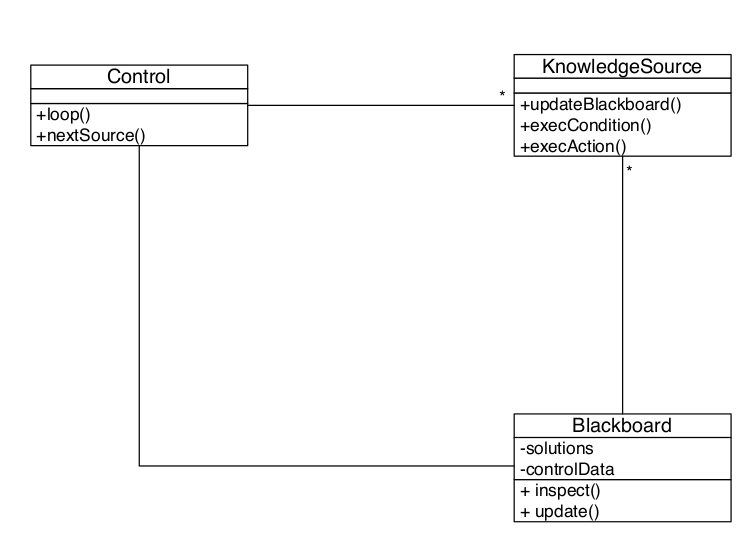
\includegraphics[width=\linewidth]{images/pattern_blackboard.png}
The knowledge sources inspect the current content of the blackboard and create new hypotheses.
Control handles the control flow of the knowledge sources.\\
The blackboard pattern is used when no algorithm for the problem is known.\\
\\
\textbf{6 Steps to Realize a Blackboard Pattern}
\begin{enumerate}
  \item Define the Problem (Identify the application domain, the requirements and the actors)
  \item Define the solution space (top-level and intermediate)
  \item Identify the knowledge sources
  \item Define the blackboard (not every information has to be understandable for every knowledge source)
  \item Define control
  \item Implement the knowledge sources (split into condition part and action part, use computational intelligence or conventional methods)
\end{enumerate}

\newpage
